\section{Evaluation} \label{sec:evaluation}

In this section, we evaluate the effectiveness of our compiler, \name{}, in scaling the performance and resource utilization of RDAs.
We first study the impact of parallelization (\ie, replicating compute and DRAMs) on applications' performance, which is measured in terms of throughput, on-chip resources (\ie, physical blocks, PBs), and off-chip bandwidth, \Cref{ssec:scalability}.
Next, we look at how various compiler optimizations (\Cref{sec:opt}) affect RDA's performance and resource utilization, as well as, the time it takes to generate the final configuration under different partitioning and merging schemes, \Cref{ssec:evalopts}. 
Finally, we compare the absolute performance of our target RDA against a Tesla V100 GPU for a mix of deep learning (DL), graph, and streaming applications, \Cref{ssec:abs-performance}.

\paragraph{Test Methodology.}
For our testbed, we modify Spatial~\cite{spatial}---a high-level language for programming accelerators---to generate the input graph, discussed in \Cref{sec:background}.
\name{} reads and processes this graph, and produces an output for our target RDA, Plasticine~\cite{plasticine}---an emerging high throughput, low-latency, and energy-efficient RDA.
We configure Plasticine in a $20\times20$ configuration, and measure its runtime using a cycle-accurate simulator.
To model DRAM, we further integrate an open-source DRAM modeling tool, called Ramulator~\cite{ramulator}, with our simulator, which adds support for an HBM2 DRAM technology, operating at \SI{1}{Tb/s}.
We also add support for a commercial optimization solver (Gurobi~\cite{gurobi}) to evaluate the solver-based graph partitioning and merging algorithms.

For performance comparison, we use a Tesla V100 GPU with a die area of \SI{815}{mm^2} using a \SI{12}{nm} technology process.
The corresponding Plasticine configuration has an area footprint of \SI{352}{mm^2} on a \SI{28}{nm} technology process,
which has 9x less transistors than the V100 GPU.
Due to speed limitations of our cycle-accurate simulation, we cannot simulate a Plasticine configuration with equivalent computing power.
And, hence, we present a normalize speedup to die area for compute-bound applications.
For writing applications, we use TensorFlow\cite{tensorflow}, compiled with cuDNN library\cite{cudnn}, for SqueezeNet and LSTM; a GPU graph library, GunRock\cite{gunrock}, for PageRank; a CUDA library for BlackScholes and sorting algorithms along with a hand-optimized implementation of a Random Forest in CUDA.

%Plasticine is a tiled-based architecture with four types of resource tiles:: Pattern Compute Unit (PCU), Pattern Memory Unit(PMU),
%DRAM Address Generator (DAG) and Memory Controller Interface (MCI).
%PCUs, PMUs, DAGs have a varying amount of reconfigurable compute resource, and each PMU contains 16 duo-ported SRAM banks.
%We select a $20\times20$ Plasticine array with an area footprint of 352$mm^2$ at the 28nm technology process.
%For Plasticine runtime, we use a cycle-accurate simulator integrated with
%ramulator\cite{ramulator} to model an HBM2 DRAM technology.
%The off-chip memory bandwidth is 1TB/s, which matches our baseline GPU.

\subsection{Scalability of RDAs}
\label{ssec:scalability}

\begin{figure*}
\centering
  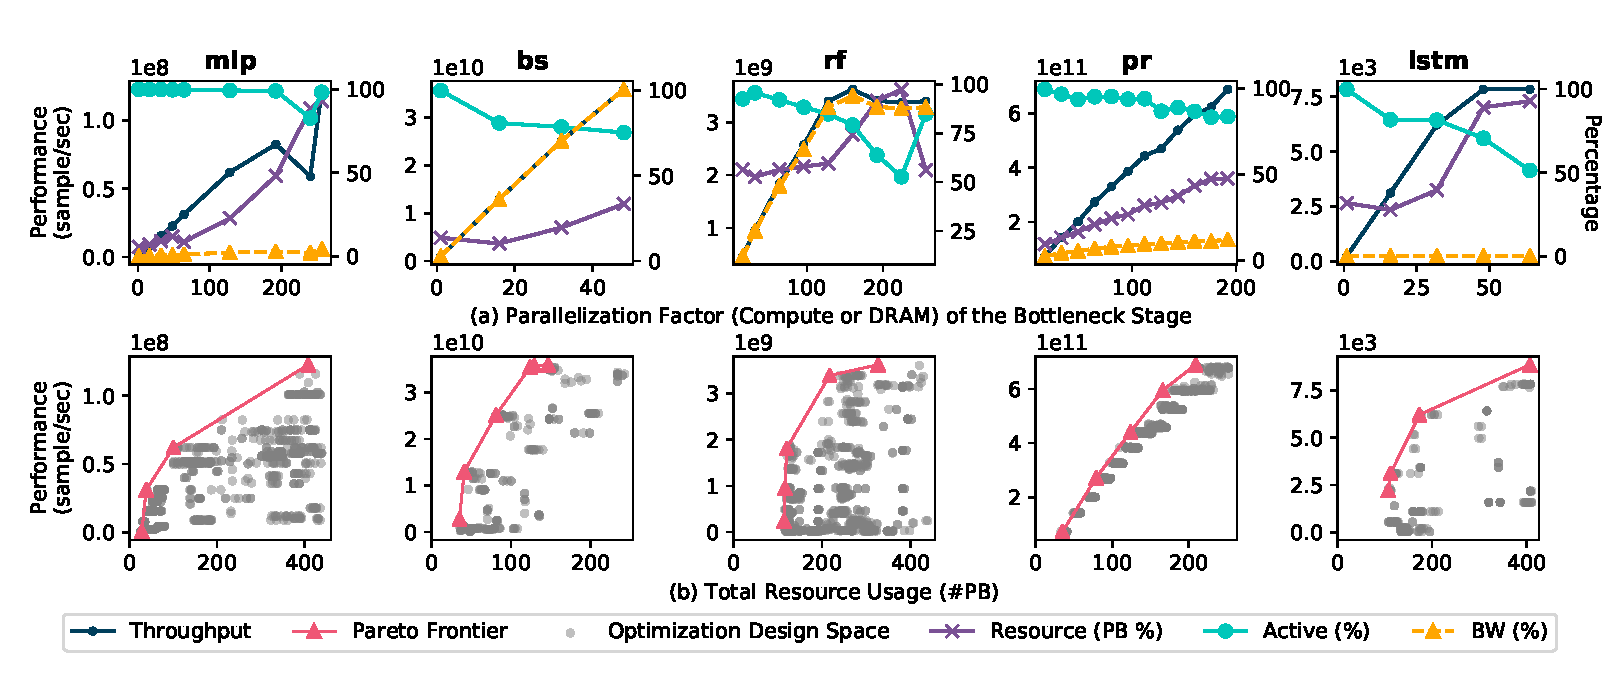
\includegraphics[width=1\textwidth]{figures/par.pdf}
  \vspace{-20pt}
  \caption{Comparing \name{}'s impact on the performance our target RDA, Plasticine, for different applications with varying parallelization factor (Top), and measuring the corresponding performance-resource tradeoff curve (Bottom).}
  \label{fig:scalability}
\end{figure*}
%\ms{Yaqi: please split legends and add a little more gap b/w the first and the second row.}

Unlike CPU-based architectures where the performance and resource utilization of a system {\em both} increase linearly with parallelization (\eg, loop unrolling a program); in RDAs, the number of resources increase sub-linearly or quadratically---depending upon the degree of program imbalance---with parallelization.
In other words, increase in resources results in super-scaler increase in performance of RDAs (\Cref{fig:scaling}).
Our experiments confirm this behavior and show that applications, when compiled with \name{}, achieve this super-linear increase in performance with respect to resources (\Cref{fig:scalability}, Bottom), while still maintaining a linear increase with respect to parallelization (\Cref{fig:scalability}, Top).   

\paragraph{Performance vs. Parallelization.}
We measure applications' throughput, on-chip resources, off-chip DRAM bandwidth, and compute activation rates at runtime, as we parallelize the bottleneck stage of an application (\Cref{fig:scalability}, Top).

% We partition and pipeline the large loop body of BlackScholes (\cemph{bb}) and all comparison trees in Random Forest inference (\cemph{rf}) across VBs, achieving high compute throughput with pipeline parallelism.
% Due to large compute bodies and complex compute graph, bs, rs, and a long short-term memory recurrent neural network inference\cite{lstm} (\cemph{lstm}) have 10--50\% resource usage without parallelization.
% \begin{figure}
%   \centering
%   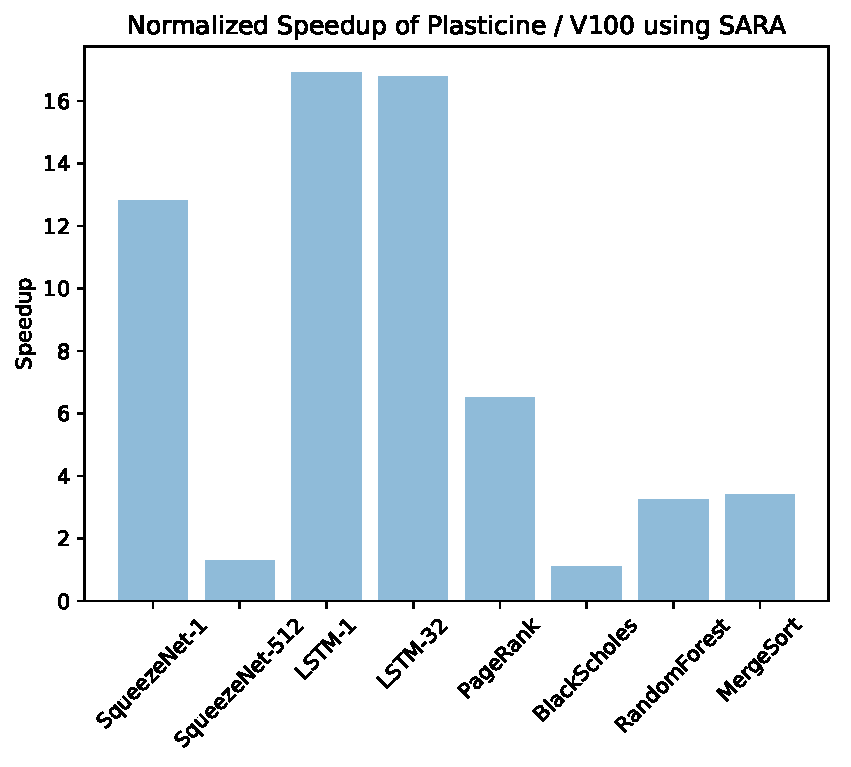
\includegraphics[width=0.8\columnwidth]{figures/speedup.pdf}
%   %\missingfigure{Incorrect synchronization}
%   \caption{Speedup}\label{fig:speedup}
%   \end{figure}
{\em Without parallelization}, \name{} can still transform an application using resource partitioning and pipelining techniques, and achieve high compute throughput.%\ms{I can't get this from the figure?}.
For example, \name{} partitions and pipelines the large loop body of BlackScholes (\Cref{fig:scalability}, Top: \cemph{\bf bs}) and all comparison trees in Random Forests (\cemph{\bf rf}), while sustaining high throughput, in tens of million samples per seconds.
On the other hand, with large compute bodies and complex graphs, \name{} can only utilize 10--50\% of resources without parallelization for \cemph{\bf bs} and \cemph{\bf rf} (as well as Long Short-Term Memory Recurrent, \cemph{\bf lstm}, neural network).

% compute-intensive apps %%% start
{\em With parallelization}, the throughput compute-intensive applications (such as Multi-Layer Perceptron (\cemph{\bf mlp}) and \cemph{\bf lstm} scales linearly until all PBs are exhausted (reaching 100\% uitilizaiton).
However, the increase in resource utilization depends on the degree of program imbalance in an application.
For example, consider an \cemph{\bf mlp} application consisting of a single batch and three layers, with previous layer having twice as many operations as the next one.
\name{} can pipeline the layers and parallelize each layer into both inner and outer channels across PBs. 
Initially, there is a small increase in resource utilization as we increase parallelization, due to unbalanced layers; however, later, the resources increase quadratically due to all-to-all communication between parallelized layers.
%\yz{Give numbering to subfigures}
Furthermore, \cemph{\bf mlp} achieves an activation rate---the percentage time a compute in the bottleneck stage is active at runtime---of about 100\% at 100\% resource usage, suggesting that \cemph{\bf mlp} incurs minimum synchronization overhead with distributed control (\Cref{sec:control}).
In the case of \cemph{\bf lstm}, there is a loop-carried dependency between multiple time steps; parallelizing the inner product of a matrix-vector multiplication within each time step, increases the initiation interval of the carried dependency due to the increase in reduction-tree depth across PBs.

For memory-intensive applications, the DRAM bandwidth directly affects their performance.
The throughput of \cemph{\bf bs} and \cemph{\bf rf} scales linearly until the DRAM bandwidth is saturated.
The DRAM load stream---that fetches features from DRAM---limits \cemph{\bf rf}'s throughput.
We see a steady increase in its throughput as \name{} parallelizes DRAM load (by loop unrolling) with minimal increase in resources---until we reach a parallelization factor of 150 (\Cref{fig:scalability}, Top), after which the resources increase linearly.
For PageRank (\cemph{\bf pr}), we observe that the DRAM coalescing buffer captures the edge locality between nearest-neighbor nodes, when parallelizing nodes' processing across PBs and (vectorize) edge processing within PBs using pull-based graphs.
Doing do, results in a dramatic reduction in off-chip memory access during sparse gather operations, thus providing a linear increase in throughput (\ie, edge/sec) until our target RDA (Plasticine) runs out of PBs with memory controller interfaces.

We observe that for most applications, the resource utilization does not increase monotonically with parallelization; as for certain parallelization factors, \name{} can statically resolve bank IDs and eliminate the crossbar communication path (\eg, \cemph{\bf mlp}, consumes less resources with a parallelization factor of 256 than 240).

%The drop of throughput scaling in mlp is because the optimization combinations that provides the best scaling did not fit due to insufficient resource and resource at parallelization 240.
%The next parallelization at 256 consumes less resource because it is dividable by the data size, which results in statically resolvable bank IDs.

\begin{figure}
\centering
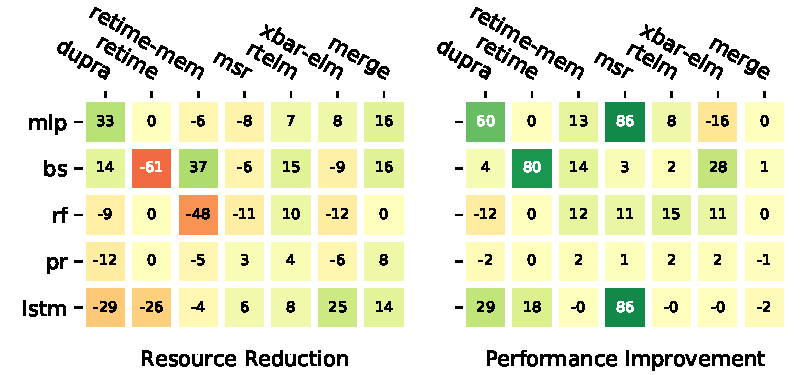
\includegraphics[width=1\columnwidth]{figures/heat.pdf}
\caption{Maximum percentage improvement in resource usage and performance for different combinations of optimizations.}
\label{fig:heat}
\centering
  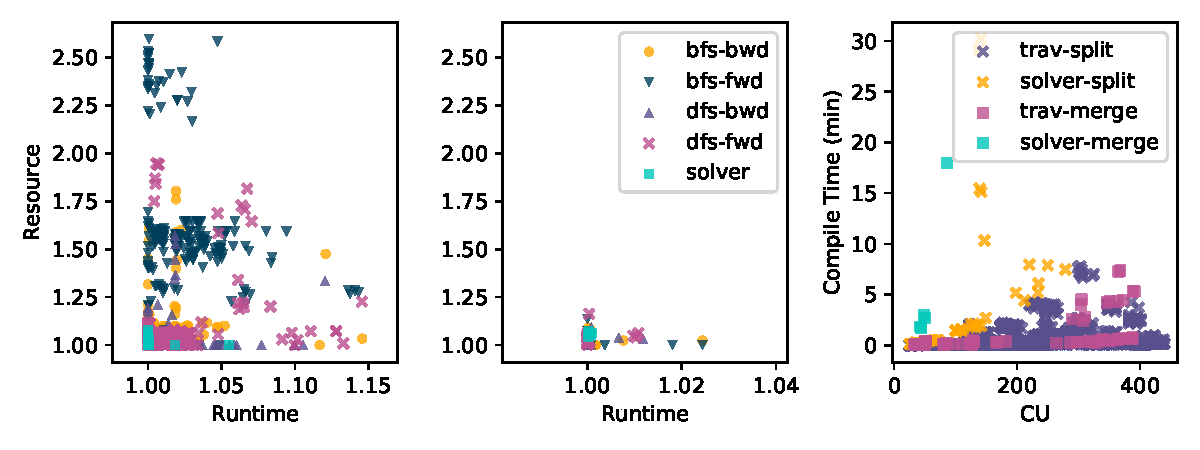
\includegraphics[width=1\columnwidth]{figures/algo.pdf}
  \caption{Normalized resource usage and runtime for traversal and solver-based partitioning and merging algorithms.}
  \label{fig:resource-runtime}
\end{figure}
%5 Table commands
\newcommand{\mrow}[1]{\multirow{2}{*}{#1}}
\newcommand{\mrowx}[1]{\multirow{3}{*}{#1}}

%\begin{table}[t]
  %\centering
    %\footnotesize
    %\begin{tabular}{llrr}
    %\toprule
      %\mrow{\bf Benchmark} & \mrow{\bf Compiler} & {\bf Latency } & {\bf Throughput} \\
                           %&                     & {\bf (ms)}     & {\bf (Inputs/s)} \\
      %\midrule
        %SqueezeNet (batch-1) & SARA                & 49.13          & 1.1        \\
        %{\em kFrames}      & TensorFlow          & 70.10          & 0.4        \\ \addlinespace
        %LSTM (batch-1)       & SARA                & 3.61           & 79.2       \\
        %{\em kSamples}     & TensorFlow          & 6.81           & 4.7        \\ \addlinespace
        %PageRank           & SARA                & 128.27         & 49         \\
        %{\em MEdges}       & GunRock             & 829.39         & 7.5        \\ \addlinespace
        %BlackScholes       & SARA                & 0.09           & 88.88      \\
        %{\em GOptions}     & CUDA                & 0.10           & 80.02      \\ \addlinespace
        %Random Forest      & SARA                & 0.10           & 1.04       \\
        %{\em MSamples}     & CUDA                & 0.32           & 0.32       \\ \addlinespace
        %Merge Sort         & SARA                & 0.63           & 6.65       \\
        %{\em GElements}    & CUDA                & 2.14           & 1.96       \\
      %\midrule
      %Speedup (Geo-Mean)  & & \textbf{2.44x} & \textbf{3.93x} \\
      %\bottomrule
    %\end{tabular}
  %\caption{Performance comparison of Plasticine (using the \name{} compiler) with Tesla's V100 GPU (using TensorFlow, GunRock, and CUDA compilers).}
  %\label{tab:gpu-comparison}
%\end{table}

\begin{table}[t]
  \centering
    \footnotesize
    \begin{tabular}{llcc}
    \toprule
      \textbf{Benchmark}       & \mrow{\bf Compiler} & {\bf Latency } & {\bf Throughput}     \\
       (Unit)                  &                     & {\bf (ms)}     & {\bf (Unit/s)}       \\
      \midrule
        SqueezeNet (batch-1)   & SARA                & 49.13          & 0.12 (1.1)           \\
        {\em (kFrames)}        & TensorFlow          & 70.10          & 0.4                  \\
                               & Speedup             & 1.43x          & 0.31x (2.75x)          \\ \addlinespace
        LSTM (batch-32)         & SARA                & 3.61           & 8.8 (79.2)           \\
        {\em (kSamples)}       & TensorFlow          & 6.81           & 4.7                  \\
                               & Speedup             & 1.89x          & 1.87x (16.85x)         \\ \addlinespace
        PageRank               & SARA                & 128.27         & 49                   \\
        {\em (MEdges)}         & GunRock             & 829.39         & 7.5                  \\
                               & Speedup             & 6.47x          & 6.5x                  \\ \addlinespace
        BlackScholes           & SARA                & 0.09           & 88.88                \\
        {\em (GOptions)}       & CUDA                & 0.10           & 80.02                \\
                               & Speedup             & 1.11x          & 1.11x                 \\ \addlinespace
        Random Forest          & SARA                & 0.10           & 1.04                 \\
        {\em (MSamples)}       & CUDA                & 0.32           & 0.32                 \\
                               & Speedup             & 3.25x          & 3.25x                 \\ \addlinespace
        Merge Sort             & SARA                & 0.63           & 6.65                 \\
        {\em (GElements)}      & CUDA                & 2.14           & 1.96                 \\
                               & Speedup             & 3.4x           & 3.4x                 \\
      \midrule
      Geo-mean Speedup         &                     & \textbf{2.44x} & \textbf{1.89x (3.93x)} \\
      \bottomrule
    \end{tabular}
  \caption{Performance comparison of Plasticine with Tesla's V100 GPU (Normalized throughput to transistor count in parentheses).}
  \label{tab:gpu-comparison}
\end{table}
  % lat_speendup = [70.1 / 49.13, 6.81 / 3.61, 829.39 / 128.27, 0.1 / 0.9, 0.32 / 0.1, 2.14 / 0.63]
  % thr_speedup = [1.1 * 1000 / 877.98, 79.2 * 1000 / 4.7 * 1000, 49 / 7.5, 88.88 / 80.02, 1.04 / 0.32, 6.65 / 1.96]
  
      %   \mrow{SqueezeNet}     & SARA    & 49.13   & 124.8 Frames/s  &  \mrow{0.14}    & \mrow{1.28}       \\
      %                         & TF      & 70.10   & 877.98 Frames/s                                       \\ \addlinespace
      %   \mrow{LSTM}           & SARA    & 3.61    & 8.8k sample/s   &  \mrow{1.87}    & \mrow{16.83}      \\
      %                         & TF      & 187.52  & 4.7k sample/s                                         \\ \addlinespace
      %   \mrow{PageRank}       & SARA    & 128.27  & 49M edge/s      &  \mrow{6.5}     & \mrow{6.5}        \\
      %                         & Gunrock & 829.39  & 7.5 M edge/s                                          \\ \addlinespace
      %   \mrow{Black Scholes}  & SARA    & 0.09    & 88.88 GOptions/s&  \mrow{1.11}    & \mrow{1.11}       \\
      %                         & Cuda    & 0.10    & 80.02 GOptions/s                                      \\ \addlinespace
      %   \mrow{Random Forest}  & SARA    & 0.10    & 1.04 Msample/s  &  \mrow{3.25}    & \mrow{3.25}       \\
      %                         & Cuda    & 0.32    & 0.32 MSamples/s                                       \\ \addlinespace
      %   \mrow{Merge Sort}     & SARA    & 0.63    & 6.65 GElements/s&  \mrow{3.39}    & \mrow{3.39}       \\
      %                         & Cuda    & 2.14    & 1.96 GElements/s                      \\
      % %   Radix Sort            & Cuda    & 1.42    & 2.96 GElements/s       \\ \addlinespace
      % %   Radix Sort            & Cuda    & 1.27    & 3.29 GElements/s       \\ \addlinespace
      % \midrule
      %   Geo-mean     & & & &     & 3.45      \\
  
  % \mrow{Local Graph Clustering, ISTA, 20 iters}                  & Plasticine & PIR     & n/a    & n/a                  &         \\
  %                                                                & V100       & Gunrock & 787.94 & n/a                  &         \\ \addlinespace
  % \mrow{SqueezeNet v1.0}
  % \mrow{LSTM, 512 units, 1 layers, 8 steps, 32 samples}, latency = 6.81ms, throughput = 4698 samples
  % \mrow{PageRank, 50 iters, delaunay\_n20 dataset}
  % \mrow{Black Scholes, 8M options}
  % \mrow{Random Forest, 102400 samples, 128 features, tree depth and number of nodes
  % \mrow{Merge Sort, 4Mi elements}
  % Radix Sort, float key, 4Mi elements
  % Radix Sort, int key, 4Mi elements
  %\begin{table*}[ht]
  %\centering
    %\small
    %\begin{tabular}{@{} llllrr *{2}{r} @{}}
    %\toprule
      %\multirow{2}{*}{\textbf{Benchmark}} & \textbf{Compiler} & \textbf{Latency (ms)} & \textbf{Throughput} &\textbf{Speedup(x)} &\textbf{Speedup, normalized (x)}\\
      %\midrule
        %\mrow{SqueezeNet}     & SARA    & 49.13   & 124.8 Frames/s  &  \mrow{0.14}    & \mrow{1.28}       \\
                              %& TF      & 70.10   & 877.98 Frames/s                                        \\ \addlinespace
        %\mrow{LSTM}           & SARA    & 3.61    & 8.8k sample/s   &  \mrow{51.76}   & \mrow{465.84}       \\
                              %& TF      & 187.52  & 170 sample/s                                           \\ \addlinespace
        %\mrow{PageRank}       & SARA    & 128.27  & 49M edge/s      &  \mrow{6.5}     & \mrow{6.5}        \\
                              %& Gunrock & 829.39  & 7.5 M edge/s                                           \\ \addlinespace
        %\mrow{Black Scholes}  & SARA    & 0.09    & 88.88 GOptions/s&  \mrow{1.11}    & \mrow{1.11}        \\
                              %& Cuda    & 0.10    & 80.02 GOptions/s                                       \\ \addlinespace
        %\mrow{Random Forest}  & SARA    & 0.10    & 1.04 Msample/s  &  \mrow{3.25}    & \mrow{3.25}       \\
                              %& Cuda    & 0.32    & 0.32 MSamples/s                                        \\ \addlinespace
        %\mrow{Merge Sort}     & SARA    & 0.63    & 6.65 GElements/s&  \mrow{3.39}    & \mrow{3.39}       \\
                              %& Cuda    & 2.14    & 1.96 GElements/s                      \\
      %\midrule
        %Geo-mean     & & & &  5.54    & 49.86      \\
      %\bottomrule
      %\addlinespace
    %\end{tabular}
  %\caption{Performance of Plasticine and Tesla V100 GPU}\label{tab:eval}
  %\end{table*}
  %\label{evaluations}

  %\begin{table*}[ht]
  %\centering
    %\small
    %\begin{tabular}{llccc}
    %\toprule
      %\textbf{Benchmark}              & \textbf{Compiler} & \textbf{Latency (ms)} & \textbf{Throughput} & \textbf{Speedup (x)}\\
      %\midrule
        %\mrow{SqueezeNet (batch-1)}   & SARA              & 49.13                 & 124.8 (1.1k) Frames/s      & \mrow{0.31 (2.75)}    \\
                                      %& TF                & 70.10                 & 400 Frames/s        &                       \\ \addlinespace
        %\mrow{LSTM (batch-32)}        & SARA              & 3.61                  & 8.8 (79.2) ksample/s       & \mrow{1.87 (16.85)} \\
                                      %& TF                & 6.81                  & 4.7 ksample/s        &                       \\ \addlinespace
        %\mrow{PageRank}               & SARA              & 128.27                & 49M edge/s          & \mrow{6.5}            \\
                                      %& Gunrock           & 829.39                & 7.5 M edge/s        &                       \\ \addlinespace
        %\mrow{Black Scholes}          & SARA              & 0.09                  & 88.88 GOptions/s    & \mrow{1.11}           \\
                                      %& Cuda              & 0.10                  & 80.02 GOptions/s    &                       \\ \addlinespace
        %\mrow{Random Forest}          & SARA              & 0.10                  & 1.04 Msample/s      & \mrow{3.25}           \\
                                      %& Cuda              & 0.32                  & 0.32 MSamples/s     &                       \\ \addlinespace
        %\mrow{Merge Sort}             & SARA              & 0.63                  & 6.65 GElements/s    & \mrow{3.39}           \\
                                      %& Cuda              & 2.14                  & 1.96 GElements/s    &                       \\
      %\midrule
        %Geo-mean                      &                   &                       &                     & 1.89 (3.93)          \\
      %\bottomrule
      %\addlinespace
    %\end{tabular}
  %\caption{Performance of Plasticine and Tesla V100 GPU}\label{tab:eval}
  %\end{table*}
  %\label{evaluations}

  %\begin{table*}[ht]
  %\centering
    %\small
    %\begin{tabular}{llccc}
    %\toprule
      %\textbf{Benchmark}              & \textbf{Compiler} & \textbf{Latency (ms)} & \textbf{Throughput} & \textbf{Speedup (x)}\\
      %\midrule
        %\mrow{SqueezeNet (batch-1)}   & SARA              & 49.13                 & 124.8 (1.1k) Frames/s      & \mrow{0.31 (2.75)}    \\
                                      %& TF                & 70.10                 & 400 Frames/s        &                       \\ \addlinespace
        %\mrow{LSTM (batch-32)}        & SARA              & 3.61                  & 8.8 (79.2) ksample/s       & \mrow{1.87 (16.85)} \\
                                      %& TF                & 6.81                  & 4.7 ksample/s        &                       \\ \addlinespace
        %\mrow{PageRank}               & SARA              & 128.27                & 49M edge/s          & \mrow{6.5}            \\
                                      %& Gunrock           & 829.39                & 7.5 M edge/s        &                       \\ \addlinespace
        %\mrow{Black Scholes}          & SARA              & 0.09                  & 88.88 GOptions/s    & \mrow{1.11}           \\
                                      %& Cuda              & 0.10                  & 80.02 GOptions/s    &                       \\ \addlinespace
        %\mrow{Random Forest}          & SARA              & 0.10                  & 1.04 Msample/s      & \mrow{3.25}           \\
                                      %& Cuda              & 0.32                  & 0.32 MSamples/s     &                       \\ \addlinespace
        %\mrow{Merge Sort}             & SARA              & 0.63                  & 6.65 GElements/s    & \mrow{3.39}           \\
                                      %& Cuda              & 2.14                  & 1.96 GElements/s    &                       \\
      %\midrule
        %Geo-mean                      &                   &                       &                     & 1.89 (3.93)          \\
      %\bottomrule
      %\addlinespace
    %\end{tabular}
  %\caption{Performance of Plasticine and Tesla V100 GPU}\label{tab:eval}
  %\end{table*}
  %\label{evaluations}



\paragraph{Performance vs. Resource Usage.}
\Cref{fig:scalability} (Bottom) shows the throughput of our target RDA, normalized to the allocated on-chip resources.
The gray dots indicate design points with varying combinations of compiler flags (\ie, optimizations turned on or off), while the Pareto Frontier (in pink) shows the best combination of these flags.
The Pareto Frontier confirms that RDAs indeed have a super-scaling relationship between performance and resources, as discussed in \Cref{sec:background}, for applications with significant program imbalance.
\cemph{\bf rf}, on the other hand, does not contain a heavily unbalanced program and, therefore, its performance can only scale linearly with resource usage at best.
The large variation in throughput within the design space (\ie, gray points) indicates that super scaling demands a collaborative effort in building new hardware and software optimizations.

\subsection{Effectiveness of Compiler Optimizations}
\label{ssec:evalopts}
In this section, we evaluate the effectiveness of compiler optimizations (\Cref{sec:opt}), as well as compare the traversal versus solver-based partitioning and merging algorithms.

\paragraph{Impact of optimizations.}
We evaluates the effectiveness of optimizations described in \Cref{sec:opt} on improving applications' resource usage and performance.
As improvements due to compiler optimizations are non-additive, we pick the most feasible combination of these optimizations for each application and then enable and disable a given optimization to measure its impact on performance and resource usage (\Cref{fig:heat}).
Each application has a large design space and as most optimizations are effective at higher levels of parallelization, we report a design point that has the maximum impact, either positively or negatively.
\emph{merge} and \emph{rtelm} are optimizations that gives a consistent resource improvement for most applications.
\emph{dupra} and \emph{msr} helps \emph{\bf mlp} and \cemph{\bf lstm}, which are heavily partitioned during the memory-partitioning stage.

\emph{dupra} significantly reduces unbalancing in the data path caused due to the large merge tree generated by memory partitioning.
\emph{retime} can have significant impact on performance of the application at the cost of increase in resource usage.
Using scratchpad as a retiming buffer with \emph{retime-mem} flag can significantly reduce resource usage.

\paragraph{Traversal versus solver-based algorithms.}
\Cref{fig:resource-runtime} (a) and (b) show the resource usage and application runtime of traversal and solver-based partitioning and merging algorithms, normalized to the minimum resource and runtime for that application.
A design point on the lower left corner (\ie, at 1) indicates the best algorithm for the particular application.

\name{} implements two graph structures that are commonly used for partitioning.
(a) A dataflow graph consisting of large basic blocks, having long-lived variables that require retiming.
%There are two common graph structures for partitioning. The first type is from the data-flow graph of a large basic block, in
%which lots of temporary variables are derived from and produces a small set external live in and live out variables.
%Such graphs typically have long-live variables that require retiming.
(b) A tree structure used for merging memory requests; an ideal partitioning of these trees does not require extra retiming.
We found that the backward BFS (bfs-bwd) produces the ideal partitioning for the balanced tree, whereas the backward DFS (dfs-bwd) produces fewer partitions in general.
The backward traversal works better than the forward traversal because the graph tends to have smaller external out-degrees than in-degrees.

To speed up convergence, we use a 15\% optimality gap that stops the solver at a reasonable solution.
As we can see, the traversal based algorithm can sometimes achieve matching or even better runtime or performance than the solver.
However, each traversal-based algorithm has adversarial cases where they can be up to 2.5x worse in resource than the best possible solution.
The right most \Cref{fig:resource-runtime} shows the compile time of both types of algorithms on different applications.
In general, the solver runtime becomes quickly unscalable with a large amount of VBs.
BlackScholes with less than 200 VBs took over 20 hours using 32 threads on an Intel Xeon Processor E7 server machine.
In practice, we can only invoke the expensive solver only when the traversal solution is insufficient, which can be
measured by the amount of slack resource in resulting partitions.

% optimization heat map ... talk about here. Figure 9.

%\ms{update the last plot to show compile time and add captions (a), (b), (c) etc to them too?}

\subsection{Comparison with a Tesla V100 GPU}
\label{ssec:abs-performance}
\Cref{tab:gpu-comparison} shows the runtime latency and throughput of Plasticine against a Tesla V100 GPU.

\paragraph{Neural Networks} Comparing to a similar TensorFlow implemenation served on V100, SqueezeNet 1.0 implemented in \name{} and served on Plasticine shows 1.5x latency speedup. It also shows 2.75x higher throughput.
SqueezeNet benefits from the flexible degrees of parallelism \name{} exploits. \name can unroll any layer of the 6-level nested loops in the convolution layer and distribute them across PBs. As such, SqueezeNet can benefit from pipeline, channel, kernel, and task-level parallelism.
In contrast, V100 only exploits data-level parallelism. Hence, SqueezeNet on V100 needs to accumulate a large batch size to fully utilize the accelerator's computation power and memory bandwidth. We also implemented a 1-layer, 8-step LSTM with 512 hidden units with SARA using the approach detailed in \cite{tz_rnn}. Our LSTM implementation achieves 1.8x latency speedup and 16.85x throughput improvement comparing to the same application served on V100.

\paragraph{BlackScholes and PageRank} We ran BlackScholes implemented in CUDA and \name till both enters steady-states. Both implementations reached similar performance due to HBM2 bandwidth limits.
PageRank implemented in \name{} Gunrock achieves 6.5x latency speedup and throughput improvement comparing to an implementation provided by Gunrock \cite{gunrock}. We found that Gunrock can only process the edge frontier set in parallel. Hence, Gunrock would not be able to fully utilize V100's compute power if the input graph is sparse.
In contrast, \name{} parallelizes both the edge and node processing with streaming DRAM data transfer. This feature allows us to exploit more degrees of parallelism within the PageRank algorithm. The input graph used in this application is denaulay\_n20 \cite{delaunayn20}.

\paragraph{RandomForest} We created a synthesized tree model that contains 8 estimators and 128 splits per estimator. Implementation with \name{} shows 3.2x in latency and throughput speedup comparing to one implemented in CUDA. We find that V100 drops performance when accessing the tree structure in each estimator due to bank conflicts. In contrast, \name{} allocates the tree structures of the estimators spatially onto the PBs and statically schedules all the data accesses. As such, \name{} manages to remove all the bank conflicts.

\paragraph{MergeSort} We parallelize multiple multi-way merge tree that merges multiple DRAM streams.
We use multiple iterations to incrementally multiple sorted DRAM partitions into a single sorted list, which achieves 3.4x normalized speedup in throughput than the fastest sort on GPU. Overall, MergeSort implemented in \name{} provides 3.4x latency speedup and throughput improvement.
